\chapter{Motivace}
V~této kapitole budou v~krátkosti představeny všechny důvody,
  proč a jak byl vyvinut nástroj MT-ComparEval.
Zvolená řešení pak budou více rozebrána v~následujících kapitolách.

\section{Experimenty a tasky}
Strojové překlady jsou při automatickém vyhodnocování porovnávány s~referenčním překladem
  (dále jen reference).
Vyhodnocování strojových překladačů může být zaměřeno na různé domény textu (např. novinové články, beletrie apod.) různých délek
  nebo na různé jazykové páry (např. z~angličtiny do češtiny, z~němčiny do češtiny apod.).
Aby uživatelé nástroje MT-ComparEval mohli snadno vyhodnocovat své strojové překladače na různých doménách nebo pro různé jazykové páry,
  mohou si vytvořit různé \textbf{\uv{experimenty}},
  v~rámci kterých mohou porovnávat své překlady s~příslušnými referencemi.
Obrázek \ref{img:experiments} ukazuje příklad vytvořených experimentů z~různých domén a jazykových párů.
\begin{figure}
	\center
	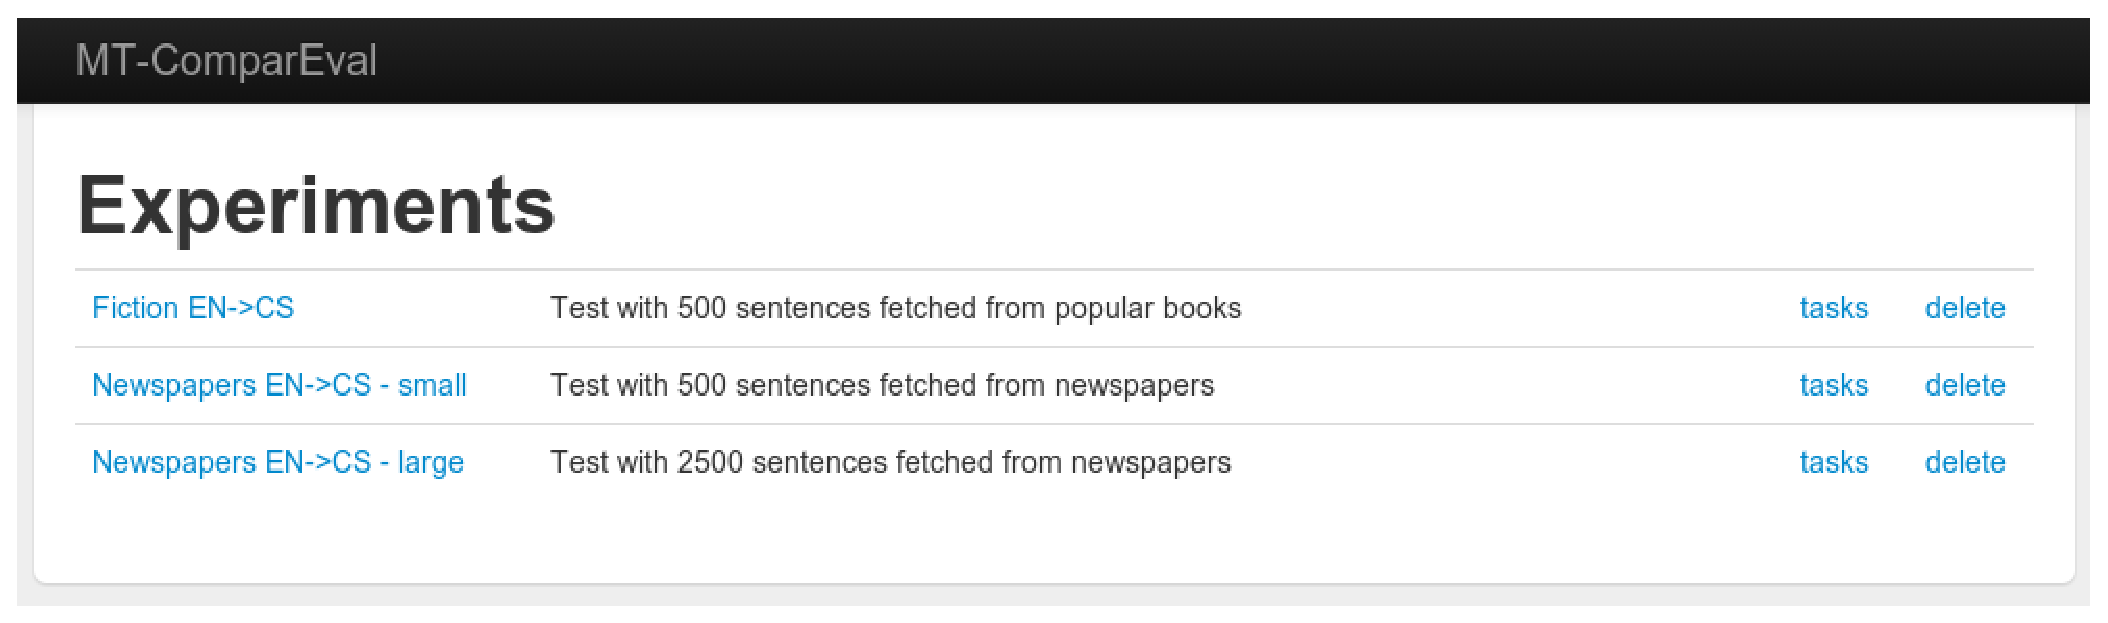
\includegraphics[width=0.9\textwidth]{img/experiments.eps}

	\caption{Přehled vytvořených experimentů v~nástroji MT-ComparEval}
	\label{img:experiments}
\end{figure}

V~každém experimentu pak uživatel může vytvářet \textbf{\uv{tasky}},
  které později může vyhodnocovat a porovnávat (viz Obrázek \ref{img:tasks}).
\begin{figure}
	\caption{Přehled vytvořených tasků v~jednom z~experimentů v~nástroji MT-ComparEval}
	\label{img:tasks}
\end{figure}

Experimenty, tasky a jiné pojmy podrobněji rozebírá ~\ref{chap:experiments}.~kapitola.


\section{Metriky strojového překladu}
K~porovnávání překladů mohou být použity metriky strojového překladu.
V~nástroji MT-ComparEval jsou metriky počítány na úrovni celých tasků 
  (viz Obrázek \ref{img:compare_metrics_tasks})
  i na úrovni jednotlivých vět
  (viz Obrázek \ref{img:compare_metrics_sentences}).

Z vypočítaných metrik lze vytvořit grafy,
  které lépe ilustrují rozdíl v kvalitě jednotlivých překladů.
Nástroj MT-ComparEval obsahuje graf rozložení absolutního rozdílu výsledků metrik v jednotlivých větách (viz Obrázek \ref{img:chart-metrics-sentences})
  a graf zobrazující rozdíly metrik celých dokumentů získaných pomocí párového bootstrap resamplingu (viz Obrázek \ref{img:chart-metrics-bs}).

Metrikami strojových překladů se více zabývá \ref{chap:metrics}. kapitola.
V~té budou představeny všechny metriky,
  které jsou použity v~nástroji MT-ComparEval.


\begin{figure}
	\caption{Porovnání metrik dvou tasků v~nástroji MT-ComparEval.}
	\label{img:compare_metrics_tasks}
\end{figure}

\begin{figure}
	\caption{Porovnání metrik dvou překladů v~nástroji MT-ComparEval.}
	\label{img:compare_metrics_sentences}
\end{figure}

\begin{figure}
	\caption{Graf zobrazující rozdělení absolutních rozdílů metrik spočtených na jednotlivých větách.}
	\label{img:chart-metrics-sentences}
\end{figure}

\begin{figure}
	\caption{Graf zobrazující rozdíly metrik získaných pomocí párového bootstrap resamplingu.}
	\label{img:chart-metrics-bs}
\end{figure}

\section{Porovnávání dvou strojových překladů}
Kvalitu strojových překladačů je možné vyhodnotit i porovnáním jednotlivých vět.
Nástroj MT-ComparEval umožňuje procházet věty seřazené podle metriky strojových překladů 
  a hledat v~těchto větách rozdíly,
  které ovlivnily výsledné metriky.
Aby uživatelé mohli snadněji vyhledat rozdíly mezi větami,
  je možné zobrazit potvrzené \mbox{n-gramy} (\mbox{n-gramy}, které se nacházeji v~referenci i strojovém překladu),
  zlepšující \mbox{n-gramy} (potvrzené \mbox{n-gramy}, které se nachází pouze v~jednom z~porovnávaných překladů)
  nebo zhoršující \mbox{n-gramy} (nepotvrzené \mbox{n-gramy}, které se nachází pouze v~jednom z~porovnávaných překladů).
Na Obrázku \ref{img:compare_sentences} je vidět porovnání dvou překladů se zvýrazněnými \mbox{n-gramy}.

Strojové překlady nemusí být porovnávány pouze na základě strojových metrik,
  další informací,
  díky které je možné si udělat lepší představu o~vlastnostech strojového překladače,
  jsou přehledy nejvíce zlepšujících a zhoršujících \mbox{n-gramů} v~jednotlivých překladech (viz Obrázek \ref{img:confirmed_ngrams}).

Přehledy zlepšujících i zhoršujicích \mbox{n-gramů} mohou být použity k~filtrování vět,
  aby si uživatel mohl snadno prohlédnout věty,
  ve kterých se dané \mbox{n-gramy} nachází.
Na Obrázku \ref{img:filtered_sentences} je vidět výpis vět obsahujících zlepšující \mbox{n-gram} ??.

\begin{figure}
	\caption{
		Porovnání dvou překladů v~nástroji MT-ComparEval.
		Pastelovými odstíny žluté a modré barvy jsou zvýrazněny potvrzené \mbox{n-gramy},
		sytými odstíny žluté a modré barvy jsou zvýrazněny zlepšující \mbox{n-gramy}
		a červenou barvou jsou zvýrazněny zhoršující \mbox{n-gramy}.
	}
	\label{img:compare_sentences}
\end{figure}

\begin{figure}
	\caption{Přehled nejvíce zlepšujících \mbox{n-gramů} v~jednotlivých překladech.}
	\label{img:confirmed_ngrams}
\end{figure}

\begin{figure}
	\caption{Výpis vět, ve kterých se nachází zlepšující \mbox{n-gram} ??}
	\label{img:filtered_sentences}
\end{figure}

O~algoritmech,
  které byly použity při porovnávání dvou překladů,
  a hledání pozic potvrzených \mbox{n-gramů}
  pojednává \ref{chap:compare}. kapitola.


\section{Automatizace a snadné použití}
Nástroj MT-ComparEval byl navržen tak,
  aby bylo možné jeho použití co nejvíce automatizovat.
Uživatelé proto nemusí ručně vytvářet každý task,
  ale mohou si napsat jednoduché skripty,
  pomocí nichž mohou vytvářet tasky v~nástroji MT-ComparEval automaticky při každé změně strojového překladače.

V~\ref{chap:users}. kapitole je možné najít informace,
  jak se používá nástroj MT-ComparEval
  a jak je možné nasadit ho do vývojového procesu.

\section{Rozšiřitelnost}
Nástroj MT-ComparEval si neklade za cíl implementovat co nejvíce metrik,
  proto jsou v~něm předprogramovány pouze některé.
Zárověň je však umožněno doprogramovat si vlastní metriky.

O~tom, jak si uživatel může doprogramovat vlastní metriky nebo jak byl nástroj MT-ComparEval vyvinut,
  je možné se dočíst v~\ref{chap:programmers}. kapitole.

